% Created by tikzDevice version 0.12.6 on 2026-07-09 15:42:22
% !TEX encoding = UTF-8 Unicode
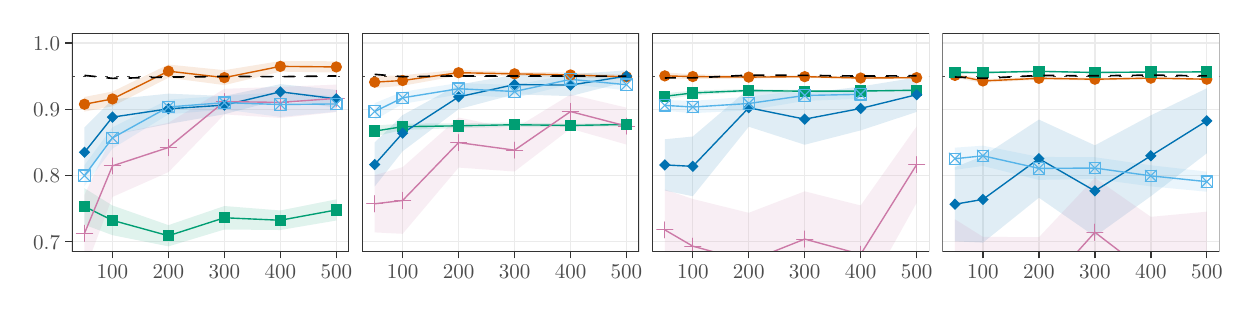
\begin{tikzpicture}[x=1pt,y=1pt]
\definecolor{fillColor}{RGB}{255,255,255}
\path[use as bounding box,fill=fillColor,fill opacity=0.00] (0,0) rectangle (433.62, 93.95);
\begin{scope}
\path[clip] (  0.00,  0.00) rectangle (433.62, 93.95);
\definecolor{drawColor}{RGB}{255,255,255}
\definecolor{fillColor}{RGB}{255,255,255}

\path[draw=drawColor,line width= 0.5pt,line join=round,line cap=round,fill=fillColor] ( -0.00,  0.00) rectangle (433.62, 93.95);
\end{scope}
\begin{scope}
\path[clip] ( 15.98, 12.99) rectangle (116.08, 91.95);
\definecolor{fillColor}{RGB}{255,255,255}

\path[fill=fillColor] ( 15.98, 12.99) rectangle (116.08, 91.95);
\definecolor{drawColor}{gray}{0.92}

\path[draw=drawColor,line width= 0.5pt,line join=round] ( 15.98, 16.58) --
	(116.08, 16.58);

\path[draw=drawColor,line width= 0.5pt,line join=round] ( 15.98, 40.50) --
	(116.08, 40.50);

\path[draw=drawColor,line width= 0.5pt,line join=round] ( 15.98, 64.43) --
	(116.08, 64.43);

\path[draw=drawColor,line width= 0.5pt,line join=round] ( 15.98, 88.36) --
	(116.08, 88.36);

\path[draw=drawColor,line width= 0.5pt,line join=round] ( 30.64, 12.99) --
	( 30.64, 91.95);

\path[draw=drawColor,line width= 0.5pt,line join=round] ( 50.87, 12.99) --
	( 50.87, 91.95);

\path[draw=drawColor,line width= 0.5pt,line join=round] ( 71.09, 12.99) --
	( 71.09, 91.95);

\path[draw=drawColor,line width= 0.5pt,line join=round] ( 91.31, 12.99) --
	( 91.31, 91.95);

\path[draw=drawColor,line width= 0.5pt,line join=round] (111.53, 12.99) --
	(111.53, 91.95);
\definecolor{drawColor}{gray}{0.30}

\path[draw=drawColor,line width= 0.4pt,dash pattern=on 1pt off 3pt ,line join=round] ( 15.98, 76.40) -- (116.08, 76.40);
\definecolor{fillColor}{RGB}{213,94,0}

\path[fill=fillColor,fill opacity=0.12] ( 20.53, 68.92) --
	( 30.64, 70.87) --
	( 50.87, 80.62) --
	( 71.09, 78.59) --
	( 91.31, 81.89) --
	(111.53, 81.80) --
	(111.53, 77.72) --
	( 91.31, 78.06) --
	( 71.09, 73.20) --
	( 50.87, 75.85) --
	( 30.64, 65.54) --
	( 20.53, 63.63) --
	cycle;

\path[] ( 20.53, 68.92) --
	( 30.64, 70.87) --
	( 50.87, 80.62) --
	( 71.09, 78.59) --
	( 91.31, 81.89) --
	(111.53, 81.80);

\path[] (111.53, 77.72) --
	( 91.31, 78.06) --
	( 71.09, 73.20) --
	( 50.87, 75.85) --
	( 30.64, 65.54) --
	( 20.53, 63.63);
\definecolor{fillColor}{RGB}{0,158,115}

\path[fill=fillColor,fill opacity=0.12] ( 20.53, 35.93) --
	( 30.64, 29.69) --
	( 50.87, 22.60) --
	( 71.09, 29.50) --
	( 91.31, 27.90) --
	(111.53, 31.91) --
	(111.53, 24.27) --
	( 91.31, 20.83) --
	( 71.09, 21.02) --
	( 50.87, 14.92) --
	( 30.64, 18.97) --
	( 20.53, 22.73) --
	cycle;

\path[] ( 20.53, 35.93) --
	( 30.64, 29.69) --
	( 50.87, 22.60) --
	( 71.09, 29.50) --
	( 91.31, 27.90) --
	(111.53, 31.91);

\path[] (111.53, 24.27) --
	( 91.31, 20.83) --
	( 71.09, 21.02) --
	( 50.87, 14.92) --
	( 30.64, 18.97) --
	( 20.53, 22.73);
\definecolor{fillColor}{RGB}{0,114,178}

\path[fill=fillColor,fill opacity=0.12] ( 20.53, 57.94) --
	( 30.64, 68.06) --
	( 50.87, 70.10) --
	( 71.09, 69.27) --
	( 91.31, 73.54) --
	(111.53, 71.48) --
	(111.53, 65.00) --
	( 91.31, 68.00) --
	( 71.09, 62.67) --
	( 50.87, 59.15) --
	( 30.64, 55.18) --
	( 20.53, 39.88) --
	cycle;

\path[] ( 20.53, 57.94) --
	( 30.64, 68.06) --
	( 50.87, 70.10) --
	( 71.09, 69.27) --
	( 91.31, 73.54) --
	(111.53, 71.48);

\path[] (111.53, 65.00) --
	( 91.31, 68.00) --
	( 71.09, 62.67) --
	( 50.87, 59.15) --
	( 30.64, 55.18) --
	( 20.53, 39.88);
\definecolor{fillColor}{RGB}{204,121,167}

\path[fill=fillColor,fill opacity=0.12] ( 20.53, 33.52) --
	( 30.64, 55.24) --
	( 50.87, 59.58) --
	( 71.09, 71.86) --
	( 91.31, 72.57) --
	(111.53, 73.37) --
	(111.53, 63.43) --
	( 91.31, 61.32) --
	( 71.09, 62.62) --
	( 50.87, 41.74) --
	( 30.64, 32.78) --
	( 20.53,  5.76) --
	cycle;

\path[] ( 20.53, 33.52) --
	( 30.64, 55.24) --
	( 50.87, 59.58) --
	( 71.09, 71.86) --
	( 91.31, 72.57) --
	(111.53, 73.37);

\path[] (111.53, 63.43) --
	( 91.31, 61.32) --
	( 71.09, 62.62) --
	( 50.87, 41.74) --
	( 30.64, 32.78) --
	( 20.53,  5.76);
\definecolor{fillColor}{RGB}{86,180,233}

\path[fill=fillColor,fill opacity=0.12] ( 20.53, 44.25) --
	( 30.64, 57.97) --
	( 50.87, 67.94) --
	( 71.09, 69.34) --
	( 91.31, 70.65) --
	(111.53, 69.19) --
	(111.53, 63.58) --
	( 91.31, 61.70) --
	( 71.09, 64.38) --
	( 50.87, 62.64) --
	( 30.64, 50.25) --
	( 20.53, 36.70) --
	cycle;

\path[] ( 20.53, 44.25) --
	( 30.64, 57.97) --
	( 50.87, 67.94) --
	( 71.09, 69.34) --
	( 91.31, 70.65) --
	(111.53, 69.19);

\path[] (111.53, 63.58) --
	( 91.31, 61.70) --
	( 71.09, 64.38) --
	( 50.87, 62.64) --
	( 30.64, 50.25) --
	( 20.53, 36.70);
\definecolor{drawColor}{RGB}{213,94,0}

\path[draw=drawColor,line width= 0.5pt,line join=round] ( 20.53, 66.28) --
	( 30.64, 68.20) --
	( 50.87, 78.23) --
	( 71.09, 75.90) --
	( 91.31, 79.97) --
	(111.53, 79.76);
\definecolor{drawColor}{RGB}{0,158,115}

\path[draw=drawColor,line width= 0.5pt,line join=round] ( 20.53, 29.33) --
	( 30.64, 24.33) --
	( 50.87, 18.76) --
	( 71.09, 25.26) --
	( 91.31, 24.36) --
	(111.53, 28.09);
\definecolor{drawColor}{RGB}{0,114,178}

\path[draw=drawColor,line width= 0.5pt,line join=round] ( 20.53, 48.91) --
	( 30.64, 61.62) --
	( 50.87, 64.63) --
	( 71.09, 65.97) --
	( 91.31, 70.77) --
	(111.53, 68.24);
\definecolor{drawColor}{RGB}{204,121,167}

\path[draw=drawColor,line width= 0.5pt,line join=round] ( 20.53, 19.64) --
	( 30.64, 44.01) --
	( 50.87, 50.66) --
	( 71.09, 67.24) --
	( 91.31, 66.95) --
	(111.53, 68.40);
\definecolor{drawColor}{RGB}{86,180,233}

\path[draw=drawColor,line width= 0.5pt,line join=round] ( 20.53, 40.48) --
	( 30.64, 54.11) --
	( 50.87, 65.29) --
	( 71.09, 66.86) --
	( 91.31, 66.18) --
	(111.53, 66.39);
\definecolor{fillColor}{RGB}{213,94,0}

\path[fill=fillColor] ( 20.53, 66.28) circle (  2.05);
\definecolor{drawColor}{RGB}{204,121,167}

\path[draw=drawColor,line width= 0.4pt,line join=round,line cap=round] ( 17.63, 19.64) -- ( 23.43, 19.64);

\path[draw=drawColor,line width= 0.4pt,line join=round,line cap=round] ( 20.53, 16.74) -- ( 20.53, 22.54);
\definecolor{fillColor}{RGB}{0,158,115}

\path[fill=fillColor] ( 18.48, 27.28) --
	( 22.58, 27.28) --
	( 22.58, 31.38) --
	( 18.48, 31.38) --
	cycle;
\definecolor{fillColor}{RGB}{0,114,178}

\path[fill=fillColor] ( 18.48, 48.91) --
	( 20.53, 50.96) --
	( 22.58, 48.91) --
	( 20.53, 46.86) --
	cycle;
\definecolor{drawColor}{RGB}{86,180,233}

\path[draw=drawColor,line width= 0.4pt,line join=round,line cap=round] ( 18.48, 38.42) rectangle ( 22.58, 42.53);

\path[draw=drawColor,line width= 0.4pt,line join=round,line cap=round] ( 18.48, 38.42) -- ( 22.58, 42.53);

\path[draw=drawColor,line width= 0.4pt,line join=round,line cap=round] ( 18.48, 42.53) -- ( 22.58, 38.42);
\definecolor{fillColor}{RGB}{213,94,0}

\path[fill=fillColor] ( 30.64, 68.20) circle (  2.05);
\definecolor{drawColor}{RGB}{204,121,167}

\path[draw=drawColor,line width= 0.4pt,line join=round,line cap=round] ( 27.74, 44.01) -- ( 33.55, 44.01);

\path[draw=drawColor,line width= 0.4pt,line join=round,line cap=round] ( 30.64, 41.11) -- ( 30.64, 46.91);
\definecolor{fillColor}{RGB}{0,158,115}

\path[fill=fillColor] ( 28.59, 22.28) --
	( 32.70, 22.28) --
	( 32.70, 26.38) --
	( 28.59, 26.38) --
	cycle;
\definecolor{fillColor}{RGB}{0,114,178}

\path[fill=fillColor] ( 28.59, 61.62) --
	( 30.64, 63.67) --
	( 32.70, 61.62) --
	( 30.64, 59.57) --
	cycle;
\definecolor{drawColor}{RGB}{86,180,233}

\path[draw=drawColor,line width= 0.4pt,line join=round,line cap=round] ( 28.59, 52.06) rectangle ( 32.70, 56.16);

\path[draw=drawColor,line width= 0.4pt,line join=round,line cap=round] ( 28.59, 52.06) -- ( 32.70, 56.16);

\path[draw=drawColor,line width= 0.4pt,line join=round,line cap=round] ( 28.59, 56.16) -- ( 32.70, 52.06);
\definecolor{fillColor}{RGB}{213,94,0}

\path[fill=fillColor] ( 50.87, 78.23) circle (  2.05);
\definecolor{drawColor}{RGB}{204,121,167}

\path[draw=drawColor,line width= 0.4pt,line join=round,line cap=round] ( 47.96, 50.66) -- ( 53.77, 50.66);

\path[draw=drawColor,line width= 0.4pt,line join=round,line cap=round] ( 50.87, 47.76) -- ( 50.87, 53.56);
\definecolor{fillColor}{RGB}{0,158,115}

\path[fill=fillColor] ( 48.81, 16.71) --
	( 52.92, 16.71) --
	( 52.92, 20.81) --
	( 48.81, 20.81) --
	cycle;
\definecolor{fillColor}{RGB}{0,114,178}

\path[fill=fillColor] ( 48.81, 64.63) --
	( 50.87, 66.68) --
	( 52.92, 64.63) --
	( 50.87, 62.58) --
	cycle;
\definecolor{drawColor}{RGB}{86,180,233}

\path[draw=drawColor,line width= 0.4pt,line join=round,line cap=round] ( 48.81, 63.23) rectangle ( 52.92, 67.34);

\path[draw=drawColor,line width= 0.4pt,line join=round,line cap=round] ( 48.81, 63.23) -- ( 52.92, 67.34);

\path[draw=drawColor,line width= 0.4pt,line join=round,line cap=round] ( 48.81, 67.34) -- ( 52.92, 63.23);
\definecolor{fillColor}{RGB}{213,94,0}

\path[fill=fillColor] ( 71.09, 75.90) circle (  2.05);
\definecolor{drawColor}{RGB}{204,121,167}

\path[draw=drawColor,line width= 0.4pt,line join=round,line cap=round] ( 68.19, 67.24) -- ( 73.99, 67.24);

\path[draw=drawColor,line width= 0.4pt,line join=round,line cap=round] ( 71.09, 64.34) -- ( 71.09, 70.14);
\definecolor{fillColor}{RGB}{0,158,115}

\path[fill=fillColor] ( 69.04, 23.21) --
	( 73.14, 23.21) --
	( 73.14, 27.31) --
	( 69.04, 27.31) --
	cycle;
\definecolor{fillColor}{RGB}{0,114,178}

\path[fill=fillColor] ( 69.04, 65.97) --
	( 71.09, 68.02) --
	( 73.14, 65.97) --
	( 71.09, 63.92) --
	cycle;
\definecolor{drawColor}{RGB}{86,180,233}

\path[draw=drawColor,line width= 0.4pt,line join=round,line cap=round] ( 69.04, 64.81) rectangle ( 73.14, 68.91);

\path[draw=drawColor,line width= 0.4pt,line join=round,line cap=round] ( 69.04, 64.81) -- ( 73.14, 68.91);

\path[draw=drawColor,line width= 0.4pt,line join=round,line cap=round] ( 69.04, 68.91) -- ( 73.14, 64.81);
\definecolor{fillColor}{RGB}{213,94,0}

\path[fill=fillColor] ( 91.31, 79.97) circle (  2.05);
\definecolor{drawColor}{RGB}{204,121,167}

\path[draw=drawColor,line width= 0.4pt,line join=round,line cap=round] ( 88.41, 66.95) -- ( 94.21, 66.95);

\path[draw=drawColor,line width= 0.4pt,line join=round,line cap=round] ( 91.31, 64.05) -- ( 91.31, 69.85);
\definecolor{fillColor}{RGB}{0,158,115}

\path[fill=fillColor] ( 89.26, 22.31) --
	( 93.36, 22.31) --
	( 93.36, 26.41) --
	( 89.26, 26.41) --
	cycle;
\definecolor{fillColor}{RGB}{0,114,178}

\path[fill=fillColor] ( 89.26, 70.77) --
	( 91.31, 72.82) --
	( 93.36, 70.77) --
	( 91.31, 68.72) --
	cycle;
\definecolor{drawColor}{RGB}{86,180,233}

\path[draw=drawColor,line width= 0.4pt,line join=round,line cap=round] ( 89.26, 64.12) rectangle ( 93.36, 68.23);

\path[draw=drawColor,line width= 0.4pt,line join=round,line cap=round] ( 89.26, 64.12) -- ( 93.36, 68.23);

\path[draw=drawColor,line width= 0.4pt,line join=round,line cap=round] ( 89.26, 68.23) -- ( 93.36, 64.12);
\definecolor{fillColor}{RGB}{213,94,0}

\path[fill=fillColor] (111.53, 79.76) circle (  2.05);
\definecolor{drawColor}{RGB}{204,121,167}

\path[draw=drawColor,line width= 0.4pt,line join=round,line cap=round] (108.63, 68.40) -- (114.43, 68.40);

\path[draw=drawColor,line width= 0.4pt,line join=round,line cap=round] (111.53, 65.50) -- (111.53, 71.30);
\definecolor{fillColor}{RGB}{0,158,115}

\path[fill=fillColor] (109.48, 26.04) --
	(113.58, 26.04) --
	(113.58, 30.14) --
	(109.48, 30.14) --
	cycle;
\definecolor{fillColor}{RGB}{0,114,178}

\path[fill=fillColor] (109.48, 68.24) --
	(111.53, 70.29) --
	(113.58, 68.24) --
	(111.53, 66.19) --
	cycle;
\definecolor{drawColor}{RGB}{86,180,233}

\path[draw=drawColor,line width= 0.4pt,line join=round,line cap=round] (109.48, 64.33) rectangle (113.58, 68.44);

\path[draw=drawColor,line width= 0.4pt,line join=round,line cap=round] (109.48, 64.33) -- (113.58, 68.44);

\path[draw=drawColor,line width= 0.4pt,line join=round,line cap=round] (109.48, 68.44) -- (113.58, 64.33);
\definecolor{drawColor}{RGB}{0,0,0}

\path[draw=drawColor,line width= 0.6pt,dash pattern=on 4pt off 4pt ,line join=round] ( 20.53, 76.70) --
	( 30.64, 75.63) --
	( 50.87, 76.10) --
	( 71.09, 76.32) --
	( 91.31, 76.24) --
	(111.53, 76.51);
\definecolor{drawColor}{gray}{0.20}

\path[draw=drawColor,line width= 0.5pt,line join=round,line cap=round] ( 15.98, 12.99) rectangle (116.08, 91.95);
\end{scope}
\begin{scope}
\path[clip] (120.83, 12.99) rectangle (220.93, 91.95);
\definecolor{fillColor}{RGB}{255,255,255}

\path[fill=fillColor] (120.83, 12.99) rectangle (220.93, 91.95);
\definecolor{drawColor}{gray}{0.92}

\path[draw=drawColor,line width= 0.5pt,line join=round] (120.83, 16.58) --
	(220.93, 16.58);

\path[draw=drawColor,line width= 0.5pt,line join=round] (120.83, 40.50) --
	(220.93, 40.50);

\path[draw=drawColor,line width= 0.5pt,line join=round] (120.83, 64.43) --
	(220.93, 64.43);

\path[draw=drawColor,line width= 0.5pt,line join=round] (120.83, 88.36) --
	(220.93, 88.36);

\path[draw=drawColor,line width= 0.5pt,line join=round] (135.49, 12.99) --
	(135.49, 91.95);

\path[draw=drawColor,line width= 0.5pt,line join=round] (155.71, 12.99) --
	(155.71, 91.95);

\path[draw=drawColor,line width= 0.5pt,line join=round] (175.93, 12.99) --
	(175.93, 91.95);

\path[draw=drawColor,line width= 0.5pt,line join=round] (196.16, 12.99) --
	(196.16, 91.95);

\path[draw=drawColor,line width= 0.5pt,line join=round] (216.38, 12.99) --
	(216.38, 91.95);
\definecolor{drawColor}{gray}{0.30}

\path[draw=drawColor,line width= 0.4pt,dash pattern=on 1pt off 3pt ,line join=round] (120.83, 76.40) -- (220.93, 76.40);
\definecolor{fillColor}{RGB}{213,94,0}

\path[fill=fillColor,fill opacity=0.12] (125.38, 76.39) --
	(135.49, 76.75) --
	(155.71, 78.76) --
	(175.93, 77.91) --
	(196.16, 77.80) --
	(216.38, 76.93) --
	(216.38, 75.42) --
	(196.16, 75.93) --
	(175.93, 76.63) --
	(155.71, 76.60) --
	(135.49, 72.95) --
	(125.38, 72.15) --
	cycle;

\path[] (125.38, 76.39) --
	(135.49, 76.75) --
	(155.71, 78.76) --
	(175.93, 77.91) --
	(196.16, 77.80) --
	(216.38, 76.93);

\path[] (216.38, 75.42) --
	(196.16, 75.93) --
	(175.93, 76.63) --
	(155.71, 76.60) --
	(135.49, 72.95) --
	(125.38, 72.15);
\definecolor{fillColor}{RGB}{0,158,115}

\path[fill=fillColor,fill opacity=0.12] (125.38, 58.55) --
	(135.49, 59.31) --
	(155.71, 59.34) --
	(175.93, 59.68) --
	(196.16, 59.26) --
	(216.38, 59.52) --
	(216.38, 58.40) --
	(196.16, 57.98) --
	(175.93, 58.08) --
	(155.71, 57.63) --
	(135.49, 57.04) --
	(125.38, 54.59) --
	cycle;

\path[] (125.38, 58.55) --
	(135.49, 59.31) --
	(155.71, 59.34) --
	(175.93, 59.68) --
	(196.16, 59.26) --
	(216.38, 59.52);

\path[] (216.38, 58.40) --
	(196.16, 57.98) --
	(175.93, 58.08) --
	(155.71, 57.63) --
	(135.49, 57.04) --
	(125.38, 54.59);
\definecolor{fillColor}{RGB}{0,114,178}

\path[fill=fillColor,fill opacity=0.12] (125.38, 52.46) --
	(135.49, 62.36) --
	(155.71, 73.37) --
	(175.93, 76.92) --
	(196.16, 77.15) --
	(216.38, 78.51) --
	(216.38, 74.39) --
	(196.16, 69.22) --
	(175.93, 69.86) --
	(155.71, 64.49) --
	(135.49, 49.30) --
	(125.38, 36.53) --
	cycle;

\path[] (125.38, 52.46) --
	(135.49, 62.36) --
	(155.71, 73.37) --
	(175.93, 76.92) --
	(196.16, 77.15) --
	(216.38, 78.51);

\path[] (216.38, 74.39) --
	(196.16, 69.22) --
	(175.93, 69.86) --
	(155.71, 64.49) --
	(135.49, 49.30) --
	(125.38, 36.53);
\definecolor{fillColor}{RGB}{204,121,167}

\path[fill=fillColor,fill opacity=0.12] (125.38, 40.64) --
	(135.49, 43.55) --
	(155.71, 61.47) --
	(175.93, 57.41) --
	(196.16, 69.83) --
	(216.38, 65.05) --
	(216.38, 51.71) --
	(196.16, 57.46) --
	(175.93, 41.97) --
	(155.71, 43.39) --
	(135.49, 19.46) --
	(125.38, 19.97) --
	cycle;

\path[] (125.38, 40.64) --
	(135.49, 43.55) --
	(155.71, 61.47) --
	(175.93, 57.41) --
	(196.16, 69.83) --
	(216.38, 65.05);

\path[] (216.38, 51.71) --
	(196.16, 57.46) --
	(175.93, 41.97) --
	(155.71, 43.39) --
	(135.49, 19.46) --
	(125.38, 19.97);
\definecolor{fillColor}{RGB}{86,180,233}

\path[fill=fillColor,fill opacity=0.12] (125.38, 66.69) --
	(135.49, 70.78) --
	(155.71, 73.97) --
	(175.93, 73.21) --
	(196.16, 77.08) --
	(216.38, 75.34) --
	(216.38, 71.33) --
	(196.16, 73.49) --
	(175.93, 68.55) --
	(155.71, 69.81) --
	(135.49, 66.42) --
	(125.38, 60.58) --
	cycle;

\path[] (125.38, 66.69) --
	(135.49, 70.78) --
	(155.71, 73.97) --
	(175.93, 73.21) --
	(196.16, 77.08) --
	(216.38, 75.34);

\path[] (216.38, 71.33) --
	(196.16, 73.49) --
	(175.93, 68.55) --
	(155.71, 69.81) --
	(135.49, 66.42) --
	(125.38, 60.58);
\definecolor{drawColor}{RGB}{213,94,0}

\path[draw=drawColor,line width= 0.5pt,line join=round] (125.38, 74.27) --
	(135.49, 74.85) --
	(155.71, 77.68) --
	(175.93, 77.27) --
	(196.16, 76.87) --
	(216.38, 76.17);
\definecolor{drawColor}{RGB}{0,158,115}

\path[draw=drawColor,line width= 0.5pt,line join=round] (125.38, 56.57) --
	(135.49, 58.17) --
	(155.71, 58.48) --
	(175.93, 58.88) --
	(196.16, 58.62) --
	(216.38, 58.96);
\definecolor{drawColor}{RGB}{0,114,178}

\path[draw=drawColor,line width= 0.5pt,line join=round] (125.38, 44.49) --
	(135.49, 55.83) --
	(155.71, 68.93) --
	(175.93, 73.39) --
	(196.16, 73.19) --
	(216.38, 76.45);
\definecolor{drawColor}{RGB}{204,121,167}

\path[draw=drawColor,line width= 0.5pt,line join=round] (125.38, 30.31) --
	(135.49, 31.50) --
	(155.71, 52.43) --
	(175.93, 49.69) --
	(196.16, 63.64) --
	(216.38, 58.38);
\definecolor{drawColor}{RGB}{86,180,233}

\path[draw=drawColor,line width= 0.5pt,line join=round] (125.38, 63.64) --
	(135.49, 68.60) --
	(155.71, 71.89) --
	(175.93, 70.88) --
	(196.16, 75.28) --
	(216.38, 73.34);
\definecolor{fillColor}{RGB}{213,94,0}

\path[fill=fillColor] (125.38, 74.27) circle (  2.05);
\definecolor{drawColor}{RGB}{204,121,167}

\path[draw=drawColor,line width= 0.4pt,line join=round,line cap=round] (122.48, 30.31) -- (128.28, 30.31);

\path[draw=drawColor,line width= 0.4pt,line join=round,line cap=round] (125.38, 27.41) -- (125.38, 33.21);
\definecolor{fillColor}{RGB}{0,158,115}

\path[fill=fillColor] (123.33, 54.52) --
	(127.43, 54.52) --
	(127.43, 58.62) --
	(123.33, 58.62) --
	cycle;
\definecolor{fillColor}{RGB}{0,114,178}

\path[fill=fillColor] (123.33, 44.49) --
	(125.38, 46.54) --
	(127.43, 44.49) --
	(125.38, 42.44) --
	cycle;
\definecolor{drawColor}{RGB}{86,180,233}

\path[draw=drawColor,line width= 0.4pt,line join=round,line cap=round] (123.33, 61.59) rectangle (127.43, 65.69);

\path[draw=drawColor,line width= 0.4pt,line join=round,line cap=round] (123.33, 61.59) -- (127.43, 65.69);

\path[draw=drawColor,line width= 0.4pt,line join=round,line cap=round] (123.33, 65.69) -- (127.43, 61.59);
\definecolor{fillColor}{RGB}{213,94,0}

\path[fill=fillColor] (135.49, 74.85) circle (  2.05);
\definecolor{drawColor}{RGB}{204,121,167}

\path[draw=drawColor,line width= 0.4pt,line join=round,line cap=round] (132.59, 31.50) -- (138.39, 31.50);

\path[draw=drawColor,line width= 0.4pt,line join=round,line cap=round] (135.49, 28.60) -- (135.49, 34.41);
\definecolor{fillColor}{RGB}{0,158,115}

\path[fill=fillColor] (133.44, 56.12) --
	(137.54, 56.12) --
	(137.54, 60.23) --
	(133.44, 60.23) --
	cycle;
\definecolor{fillColor}{RGB}{0,114,178}

\path[fill=fillColor] (133.44, 55.83) --
	(135.49, 57.88) --
	(137.54, 55.83) --
	(135.49, 53.78) --
	cycle;
\definecolor{drawColor}{RGB}{86,180,233}

\path[draw=drawColor,line width= 0.4pt,line join=round,line cap=round] (133.44, 66.55) rectangle (137.54, 70.65);

\path[draw=drawColor,line width= 0.4pt,line join=round,line cap=round] (133.44, 66.55) -- (137.54, 70.65);

\path[draw=drawColor,line width= 0.4pt,line join=round,line cap=round] (133.44, 70.65) -- (137.54, 66.55);
\definecolor{fillColor}{RGB}{213,94,0}

\path[fill=fillColor] (155.71, 77.68) circle (  2.05);
\definecolor{drawColor}{RGB}{204,121,167}

\path[draw=drawColor,line width= 0.4pt,line join=round,line cap=round] (152.81, 52.43) -- (158.61, 52.43);

\path[draw=drawColor,line width= 0.4pt,line join=round,line cap=round] (155.71, 49.52) -- (155.71, 55.33);
\definecolor{fillColor}{RGB}{0,158,115}

\path[fill=fillColor] (153.66, 56.43) --
	(157.76, 56.43) --
	(157.76, 60.53) --
	(153.66, 60.53) --
	cycle;
\definecolor{fillColor}{RGB}{0,114,178}

\path[fill=fillColor] (153.66, 68.93) --
	(155.71, 70.98) --
	(157.76, 68.93) --
	(155.71, 66.88) --
	cycle;
\definecolor{drawColor}{RGB}{86,180,233}

\path[draw=drawColor,line width= 0.4pt,line join=round,line cap=round] (153.66, 69.84) rectangle (157.76, 73.94);

\path[draw=drawColor,line width= 0.4pt,line join=round,line cap=round] (153.66, 69.84) -- (157.76, 73.94);

\path[draw=drawColor,line width= 0.4pt,line join=round,line cap=round] (153.66, 73.94) -- (157.76, 69.84);
\definecolor{fillColor}{RGB}{213,94,0}

\path[fill=fillColor] (175.93, 77.27) circle (  2.05);
\definecolor{drawColor}{RGB}{204,121,167}

\path[draw=drawColor,line width= 0.4pt,line join=round,line cap=round] (173.03, 49.69) -- (178.83, 49.69);

\path[draw=drawColor,line width= 0.4pt,line join=round,line cap=round] (175.93, 46.79) -- (175.93, 52.59);
\definecolor{fillColor}{RGB}{0,158,115}

\path[fill=fillColor] (173.88, 56.83) --
	(177.99, 56.83) --
	(177.99, 60.93) --
	(173.88, 60.93) --
	cycle;
\definecolor{fillColor}{RGB}{0,114,178}

\path[fill=fillColor] (173.88, 73.39) --
	(175.93, 75.44) --
	(177.99, 73.39) --
	(175.93, 71.34) --
	cycle;
\definecolor{drawColor}{RGB}{86,180,233}

\path[draw=drawColor,line width= 0.4pt,line join=round,line cap=round] (173.88, 68.83) rectangle (177.99, 72.93);

\path[draw=drawColor,line width= 0.4pt,line join=round,line cap=round] (173.88, 68.83) -- (177.99, 72.93);

\path[draw=drawColor,line width= 0.4pt,line join=round,line cap=round] (173.88, 72.93) -- (177.99, 68.83);
\definecolor{fillColor}{RGB}{213,94,0}

\path[fill=fillColor] (196.16, 76.87) circle (  2.05);
\definecolor{drawColor}{RGB}{204,121,167}

\path[draw=drawColor,line width= 0.4pt,line join=round,line cap=round] (193.25, 63.64) -- (199.06, 63.64);

\path[draw=drawColor,line width= 0.4pt,line join=round,line cap=round] (196.16, 60.74) -- (196.16, 66.55);
\definecolor{fillColor}{RGB}{0,158,115}

\path[fill=fillColor] (194.10, 56.56) --
	(198.21, 56.56) --
	(198.21, 60.67) --
	(194.10, 60.67) --
	cycle;
\definecolor{fillColor}{RGB}{0,114,178}

\path[fill=fillColor] (194.10, 73.19) --
	(196.16, 75.24) --
	(198.21, 73.19) --
	(196.16, 71.14) --
	cycle;
\definecolor{drawColor}{RGB}{86,180,233}

\path[draw=drawColor,line width= 0.4pt,line join=round,line cap=round] (194.10, 73.23) rectangle (198.21, 77.34);

\path[draw=drawColor,line width= 0.4pt,line join=round,line cap=round] (194.10, 73.23) -- (198.21, 77.34);

\path[draw=drawColor,line width= 0.4pt,line join=round,line cap=round] (194.10, 77.34) -- (198.21, 73.23);
\definecolor{fillColor}{RGB}{213,94,0}

\path[fill=fillColor] (216.38, 76.17) circle (  2.05);
\definecolor{drawColor}{RGB}{204,121,167}

\path[draw=drawColor,line width= 0.4pt,line join=round,line cap=round] (213.48, 58.38) -- (219.28, 58.38);

\path[draw=drawColor,line width= 0.4pt,line join=round,line cap=round] (216.38, 55.48) -- (216.38, 61.28);
\definecolor{fillColor}{RGB}{0,158,115}

\path[fill=fillColor] (214.33, 56.91) --
	(218.43, 56.91) --
	(218.43, 61.01) --
	(214.33, 61.01) --
	cycle;
\definecolor{fillColor}{RGB}{0,114,178}

\path[fill=fillColor] (214.33, 76.45) --
	(216.38, 78.50) --
	(218.43, 76.45) --
	(216.38, 74.40) --
	cycle;
\definecolor{drawColor}{RGB}{86,180,233}

\path[draw=drawColor,line width= 0.4pt,line join=round,line cap=round] (214.33, 71.29) rectangle (218.43, 75.39);

\path[draw=drawColor,line width= 0.4pt,line join=round,line cap=round] (214.33, 71.29) -- (218.43, 75.39);

\path[draw=drawColor,line width= 0.4pt,line join=round,line cap=round] (214.33, 75.39) -- (218.43, 71.29);
\definecolor{drawColor}{RGB}{0,0,0}

\path[draw=drawColor,line width= 0.6pt,dash pattern=on 4pt off 4pt ,line join=round] (125.38, 77.08) --
	(135.49, 76.24) --
	(155.71, 76.52) --
	(175.93, 76.47) --
	(196.16, 76.47) --
	(216.38, 76.43);
\definecolor{drawColor}{gray}{0.20}

\path[draw=drawColor,line width= 0.5pt,line join=round,line cap=round] (120.83, 12.99) rectangle (220.93, 91.95);
\end{scope}
\begin{scope}
\path[clip] (225.68, 12.99) rectangle (325.77, 91.95);
\definecolor{fillColor}{RGB}{255,255,255}

\path[fill=fillColor] (225.68, 12.99) rectangle (325.77, 91.95);
\definecolor{drawColor}{gray}{0.92}

\path[draw=drawColor,line width= 0.5pt,line join=round] (225.68, 16.58) --
	(325.77, 16.58);

\path[draw=drawColor,line width= 0.5pt,line join=round] (225.68, 40.50) --
	(325.77, 40.50);

\path[draw=drawColor,line width= 0.5pt,line join=round] (225.68, 64.43) --
	(325.77, 64.43);

\path[draw=drawColor,line width= 0.5pt,line join=round] (225.68, 88.36) --
	(325.77, 88.36);

\path[draw=drawColor,line width= 0.5pt,line join=round] (240.34, 12.99) --
	(240.34, 91.95);

\path[draw=drawColor,line width= 0.5pt,line join=round] (260.56, 12.99) --
	(260.56, 91.95);

\path[draw=drawColor,line width= 0.5pt,line join=round] (280.78, 12.99) --
	(280.78, 91.95);

\path[draw=drawColor,line width= 0.5pt,line join=round] (301.00, 12.99) --
	(301.00, 91.95);

\path[draw=drawColor,line width= 0.5pt,line join=round] (321.22, 12.99) --
	(321.22, 91.95);
\definecolor{drawColor}{gray}{0.30}

\path[draw=drawColor,line width= 0.4pt,dash pattern=on 1pt off 3pt ,line join=round] (225.68, 76.40) -- (325.77, 76.40);
\definecolor{fillColor}{RGB}{213,94,0}

\path[fill=fillColor,fill opacity=0.12] (230.23, 77.77) --
	(240.34, 77.13) --
	(260.56, 76.64) --
	(280.78, 76.69) --
	(301.00, 76.21) --
	(321.22, 76.24) --
	(321.22, 75.53) --
	(301.00, 75.29) --
	(280.78, 75.81) --
	(260.56, 75.52) --
	(240.34, 75.43) --
	(230.23, 75.30) --
	cycle;

\path[] (230.23, 77.77) --
	(240.34, 77.13) --
	(260.56, 76.64) --
	(280.78, 76.69) --
	(301.00, 76.21) --
	(321.22, 76.24);

\path[] (321.22, 75.53) --
	(301.00, 75.29) --
	(280.78, 75.81) --
	(260.56, 75.52) --
	(240.34, 75.43) --
	(230.23, 75.30);
\definecolor{fillColor}{RGB}{0,158,115}

\path[fill=fillColor,fill opacity=0.12] (230.23, 70.25) --
	(240.34, 71.23) --
	(260.56, 71.75) --
	(280.78, 71.42) --
	(301.00, 71.41) --
	(321.22, 71.62) --
	(321.22, 71.05) --
	(301.00, 70.68) --
	(280.78, 70.55) --
	(260.56, 70.72) --
	(240.34, 69.52) --
	(230.23, 68.05) --
	cycle;

\path[] (230.23, 70.25) --
	(240.34, 71.23) --
	(260.56, 71.75) --
	(280.78, 71.42) --
	(301.00, 71.41) --
	(321.22, 71.62);

\path[] (321.22, 71.05) --
	(301.00, 70.68) --
	(280.78, 70.55) --
	(260.56, 70.72) --
	(240.34, 69.52) --
	(230.23, 68.05);
\definecolor{fillColor}{RGB}{0,114,178}

\path[fill=fillColor,fill opacity=0.12] (230.23, 53.62) --
	(240.34, 54.62) --
	(260.56, 71.87) --
	(280.78, 70.13) --
	(301.00, 72.68) --
	(321.22, 75.96) --
	(321.22, 63.50) --
	(301.00, 56.83) --
	(280.78, 51.65) --
	(260.56, 58.15) --
	(240.34, 33.04) --
	(230.23, 35.09) --
	cycle;

\path[] (230.23, 53.62) --
	(240.34, 54.62) --
	(260.56, 71.87) --
	(280.78, 70.13) --
	(301.00, 72.68) --
	(321.22, 75.96);

\path[] (321.22, 63.50) --
	(301.00, 56.83) --
	(280.78, 51.65) --
	(260.56, 58.15) --
	(240.34, 33.04) --
	(230.23, 35.09);
\definecolor{fillColor}{RGB}{204,121,167}

\path[fill=fillColor,fill opacity=0.12] (230.23, 35.47) --
	(240.34, 32.05) --
	(260.56, 27.05) --
	(280.78, 34.81) --
	(301.00, 29.70) --
	(321.22, 58.25) --
	(321.22, 30.64) --
	(301.00, -5.57) --
	(280.78,  0.31) --
	(260.56, -8.08) --
	(240.34, -2.07) --
	(230.23,  6.29) --
	cycle;

\path[] (230.23, 35.47) --
	(240.34, 32.05) --
	(260.56, 27.05) --
	(280.78, 34.81) --
	(301.00, 29.70) --
	(321.22, 58.25);

\path[] (321.22, 30.64) --
	(301.00, -5.57) --
	(280.78,  0.31) --
	(260.56, -8.08) --
	(240.34, -2.07) --
	(230.23,  6.29);
\definecolor{fillColor}{RGB}{86,180,233}

\path[fill=fillColor,fill opacity=0.12] (230.23, 67.82) --
	(240.34, 67.50) --
	(260.56, 69.01) --
	(280.78, 71.41) --
	(301.00, 71.44) --
	(301.00, 68.27) --
	(280.78, 67.49) --
	(260.56, 64.08) --
	(240.34, 63.05) --
	(230.23, 63.92) --
	cycle;

\path[] (230.23, 67.82) --
	(240.34, 67.50) --
	(260.56, 69.01) --
	(280.78, 71.41) --
	(301.00, 71.44);

\path[] (301.00, 68.27) --
	(280.78, 67.49) --
	(260.56, 64.08) --
	(240.34, 63.05) --
	(230.23, 63.92);
\definecolor{drawColor}{RGB}{213,94,0}

\path[draw=drawColor,line width= 0.5pt,line join=round] (230.23, 76.53) --
	(240.34, 76.28) --
	(260.56, 76.08) --
	(280.78, 76.25) --
	(301.00, 75.75) --
	(321.22, 75.89);
\definecolor{drawColor}{RGB}{0,158,115}

\path[draw=drawColor,line width= 0.5pt,line join=round] (230.23, 69.15) --
	(240.34, 70.37) --
	(260.56, 71.24) --
	(280.78, 70.99) --
	(301.00, 71.05) --
	(321.22, 71.34);
\definecolor{drawColor}{RGB}{0,114,178}

\path[draw=drawColor,line width= 0.5pt,line join=round] (230.23, 44.36) --
	(240.34, 43.83) --
	(260.56, 65.01) --
	(280.78, 60.89) --
	(301.00, 64.76) --
	(321.22, 69.73);
\definecolor{drawColor}{RGB}{204,121,167}

\path[draw=drawColor,line width= 0.5pt,line join=round] (230.23, 20.88) --
	(240.34, 14.99) --
	(260.56,  9.49) --
	(280.78, 17.56) --
	(301.00, 12.06) --
	(321.22, 44.45);
\definecolor{drawColor}{RGB}{86,180,233}

\path[draw=drawColor,line width= 0.5pt,line join=round] (230.23, 65.87) --
	(240.34, 65.28) --
	(260.56, 66.55) --
	(280.78, 69.45) --
	(301.00, 69.86);
\definecolor{fillColor}{RGB}{213,94,0}

\path[fill=fillColor] (230.23, 76.53) circle (  2.05);
\definecolor{drawColor}{RGB}{204,121,167}

\path[draw=drawColor,line width= 0.4pt,line join=round,line cap=round] (227.33, 20.88) -- (233.13, 20.88);

\path[draw=drawColor,line width= 0.4pt,line join=round,line cap=round] (230.23, 17.98) -- (230.23, 23.78);
\definecolor{fillColor}{RGB}{0,158,115}

\path[fill=fillColor] (228.18, 67.09) --
	(232.28, 67.09) --
	(232.28, 71.20) --
	(228.18, 71.20) --
	cycle;
\definecolor{fillColor}{RGB}{0,114,178}

\path[fill=fillColor] (228.18, 44.36) --
	(230.23, 46.41) --
	(232.28, 44.36) --
	(230.23, 42.30) --
	cycle;
\definecolor{drawColor}{RGB}{86,180,233}

\path[draw=drawColor,line width= 0.4pt,line join=round,line cap=round] (228.18, 63.82) rectangle (232.28, 67.92);

\path[draw=drawColor,line width= 0.4pt,line join=round,line cap=round] (228.18, 63.82) -- (232.28, 67.92);

\path[draw=drawColor,line width= 0.4pt,line join=round,line cap=round] (228.18, 67.92) -- (232.28, 63.82);
\definecolor{fillColor}{RGB}{213,94,0}

\path[fill=fillColor] (240.34, 76.28) circle (  2.05);
\definecolor{drawColor}{RGB}{204,121,167}

\path[draw=drawColor,line width= 0.4pt,line join=round,line cap=round] (237.44, 14.99) -- (243.24, 14.99);

\path[draw=drawColor,line width= 0.4pt,line join=round,line cap=round] (240.34, 12.09) -- (240.34, 17.89);
\definecolor{fillColor}{RGB}{0,158,115}

\path[fill=fillColor] (238.29, 68.32) --
	(242.39, 68.32) --
	(242.39, 72.43) --
	(238.29, 72.43) --
	cycle;
\definecolor{fillColor}{RGB}{0,114,178}

\path[fill=fillColor] (238.29, 43.83) --
	(240.34, 45.88) --
	(242.39, 43.83) --
	(240.34, 41.78) --
	cycle;
\definecolor{drawColor}{RGB}{86,180,233}

\path[draw=drawColor,line width= 0.4pt,line join=round,line cap=round] (238.29, 63.23) rectangle (242.39, 67.33);

\path[draw=drawColor,line width= 0.4pt,line join=round,line cap=round] (238.29, 63.23) -- (242.39, 67.33);

\path[draw=drawColor,line width= 0.4pt,line join=round,line cap=round] (238.29, 67.33) -- (242.39, 63.23);
\definecolor{fillColor}{RGB}{213,94,0}

\path[fill=fillColor] (260.56, 76.08) circle (  2.05);
\definecolor{drawColor}{RGB}{204,121,167}

\path[draw=drawColor,line width= 0.4pt,line join=round,line cap=round] (257.66,  9.49) -- (263.46,  9.49);

\path[draw=drawColor,line width= 0.4pt,line join=round,line cap=round] (260.56,  6.59) -- (260.56, 12.39);
\definecolor{fillColor}{RGB}{0,158,115}

\path[fill=fillColor] (258.51, 69.18) --
	(262.61, 69.18) --
	(262.61, 73.29) --
	(258.51, 73.29) --
	cycle;
\definecolor{fillColor}{RGB}{0,114,178}

\path[fill=fillColor] (258.51, 65.01) --
	(260.56, 67.06) --
	(262.61, 65.01) --
	(260.56, 62.96) --
	cycle;
\definecolor{drawColor}{RGB}{86,180,233}

\path[draw=drawColor,line width= 0.4pt,line join=round,line cap=round] (258.51, 64.50) rectangle (262.61, 68.60);

\path[draw=drawColor,line width= 0.4pt,line join=round,line cap=round] (258.51, 64.50) -- (262.61, 68.60);

\path[draw=drawColor,line width= 0.4pt,line join=round,line cap=round] (258.51, 68.60) -- (262.61, 64.50);
\definecolor{fillColor}{RGB}{213,94,0}

\path[fill=fillColor] (280.78, 76.25) circle (  2.05);
\definecolor{drawColor}{RGB}{204,121,167}

\path[draw=drawColor,line width= 0.4pt,line join=round,line cap=round] (277.88, 17.56) -- (283.68, 17.56);

\path[draw=drawColor,line width= 0.4pt,line join=round,line cap=round] (280.78, 14.65) -- (280.78, 20.46);
\definecolor{fillColor}{RGB}{0,158,115}

\path[fill=fillColor] (278.73, 68.94) --
	(282.83, 68.94) --
	(282.83, 73.04) --
	(278.73, 73.04) --
	cycle;
\definecolor{fillColor}{RGB}{0,114,178}

\path[fill=fillColor] (278.73, 60.89) --
	(280.78, 62.94) --
	(282.83, 60.89) --
	(280.78, 58.84) --
	cycle;
\definecolor{drawColor}{RGB}{86,180,233}

\path[draw=drawColor,line width= 0.4pt,line join=round,line cap=round] (278.73, 67.40) rectangle (282.83, 71.50);

\path[draw=drawColor,line width= 0.4pt,line join=round,line cap=round] (278.73, 67.40) -- (282.83, 71.50);

\path[draw=drawColor,line width= 0.4pt,line join=round,line cap=round] (278.73, 71.50) -- (282.83, 67.40);
\definecolor{fillColor}{RGB}{213,94,0}

\path[fill=fillColor] (301.00, 75.75) circle (  2.05);
\definecolor{drawColor}{RGB}{204,121,167}

\path[draw=drawColor,line width= 0.4pt,line join=round,line cap=round] (298.10, 12.06) -- (303.90, 12.06);

\path[draw=drawColor,line width= 0.4pt,line join=round,line cap=round] (301.00,  9.16) -- (301.00, 14.96);
\definecolor{fillColor}{RGB}{0,158,115}

\path[fill=fillColor] (298.95, 68.99) --
	(303.05, 68.99) --
	(303.05, 73.10) --
	(298.95, 73.10) --
	cycle;
\definecolor{fillColor}{RGB}{0,114,178}

\path[fill=fillColor] (298.95, 64.76) --
	(301.00, 66.81) --
	(303.05, 64.76) --
	(301.00, 62.71) --
	cycle;
\definecolor{drawColor}{RGB}{86,180,233}

\path[draw=drawColor,line width= 0.4pt,line join=round,line cap=round] (298.95, 67.81) rectangle (303.05, 71.91);

\path[draw=drawColor,line width= 0.4pt,line join=round,line cap=round] (298.95, 67.81) -- (303.05, 71.91);

\path[draw=drawColor,line width= 0.4pt,line join=round,line cap=round] (298.95, 71.91) -- (303.05, 67.81);
\definecolor{fillColor}{RGB}{213,94,0}

\path[fill=fillColor] (321.22, 75.89) circle (  2.05);
\definecolor{drawColor}{RGB}{204,121,167}

\path[draw=drawColor,line width= 0.4pt,line join=round,line cap=round] (318.32, 44.45) -- (324.12, 44.45);

\path[draw=drawColor,line width= 0.4pt,line join=round,line cap=round] (321.22, 41.55) -- (321.22, 47.35);
\definecolor{fillColor}{RGB}{0,158,115}

\path[fill=fillColor] (319.17, 69.28) --
	(323.27, 69.28) --
	(323.27, 73.39) --
	(319.17, 73.39) --
	cycle;
\definecolor{fillColor}{RGB}{0,114,178}

\path[fill=fillColor] (319.17, 69.73) --
	(321.22, 71.78) --
	(323.27, 69.73) --
	(321.22, 67.68) --
	cycle;
\definecolor{drawColor}{RGB}{0,0,0}

\path[draw=drawColor,line width= 0.6pt,dash pattern=on 4pt off 4pt ,line join=round] (230.23, 75.79) --
	(240.34, 75.82) --
	(260.56, 76.78) --
	(280.78, 76.71) --
	(301.00, 76.47) --
	(321.22, 76.56);
\definecolor{drawColor}{gray}{0.20}

\path[draw=drawColor,line width= 0.5pt,line join=round,line cap=round] (225.68, 12.99) rectangle (325.77, 91.95);
\end{scope}
\begin{scope}
\path[clip] (330.52, 12.99) rectangle (430.62, 91.95);
\definecolor{fillColor}{RGB}{255,255,255}

\path[fill=fillColor] (330.52, 12.99) rectangle (430.62, 91.95);
\definecolor{drawColor}{gray}{0.92}

\path[draw=drawColor,line width= 0.5pt,line join=round] (330.52, 16.58) --
	(430.62, 16.58);

\path[draw=drawColor,line width= 0.5pt,line join=round] (330.52, 40.50) --
	(430.62, 40.50);

\path[draw=drawColor,line width= 0.5pt,line join=round] (330.52, 64.43) --
	(430.62, 64.43);

\path[draw=drawColor,line width= 0.5pt,line join=round] (330.52, 88.36) --
	(430.62, 88.36);

\path[draw=drawColor,line width= 0.5pt,line join=round] (345.18, 12.99) --
	(345.18, 91.95);

\path[draw=drawColor,line width= 0.5pt,line join=round] (365.41, 12.99) --
	(365.41, 91.95);

\path[draw=drawColor,line width= 0.5pt,line join=round] (385.63, 12.99) --
	(385.63, 91.95);

\path[draw=drawColor,line width= 0.5pt,line join=round] (405.85, 12.99) --
	(405.85, 91.95);

\path[draw=drawColor,line width= 0.5pt,line join=round] (426.07, 12.99) --
	(426.07, 91.95);
\definecolor{drawColor}{gray}{0.30}

\path[draw=drawColor,line width= 0.4pt,dash pattern=on 1pt off 3pt ,line join=round] (330.52, 76.40) -- (430.62, 76.40);
\definecolor{fillColor}{RGB}{213,94,0}

\path[fill=fillColor,fill opacity=0.12] (335.07, 77.60) --
	(345.18, 75.37) --
	(365.41, 76.15) --
	(385.63, 75.78) --
	(405.85, 76.09) --
	(426.07, 75.64) --
	(426.07, 75.02) --
	(405.85, 75.34) --
	(385.63, 74.86) --
	(365.41, 75.15) --
	(345.18, 74.02) --
	(335.07, 75.80) --
	cycle;

\path[] (335.07, 77.60) --
	(345.18, 75.37) --
	(365.41, 76.15) --
	(385.63, 75.78) --
	(405.85, 76.09) --
	(426.07, 75.64);

\path[] (426.07, 75.02) --
	(405.85, 75.34) --
	(385.63, 74.86) --
	(365.41, 75.15) --
	(345.18, 74.02) --
	(335.07, 75.80);
\definecolor{fillColor}{RGB}{0,158,115}

\path[fill=fillColor,fill opacity=0.12] (335.07, 78.42) --
	(345.18, 78.13) --
	(365.41, 78.48) --
	(385.63, 77.99) --
	(405.85, 78.12) --
	(426.07, 78.15) --
	(426.07, 77.77) --
	(405.85, 77.73) --
	(385.63, 77.51) --
	(365.41, 77.86) --
	(345.18, 77.34) --
	(335.07, 77.20) --
	cycle;

\path[] (335.07, 78.42) --
	(345.18, 78.13) --
	(365.41, 78.48) --
	(385.63, 77.99) --
	(405.85, 78.12) --
	(426.07, 78.15);

\path[] (426.07, 77.77) --
	(405.85, 77.73) --
	(385.63, 77.51) --
	(365.41, 77.86) --
	(345.18, 77.34) --
	(335.07, 77.20);
\definecolor{fillColor}{RGB}{0,114,178}

\path[fill=fillColor,fill opacity=0.12] (335.07, 43.56) --
	(345.18, 47.53) --
	(365.41, 60.74) --
	(385.63, 51.43) --
	(405.85, 62.26) --
	(426.07, 72.03) --
	(426.07, 48.55) --
	(405.85, 33.04) --
	(385.63, 18.49) --
	(365.41, 32.50) --
	(345.18, 16.27) --
	(335.07, 16.75) --
	cycle;

\path[] (335.07, 43.56) --
	(345.18, 47.53) --
	(365.41, 60.74) --
	(385.63, 51.43) --
	(405.85, 62.26) --
	(426.07, 72.03);

\path[] (426.07, 48.55) --
	(405.85, 33.04) --
	(385.63, 18.49) --
	(365.41, 32.50) --
	(345.18, 16.27) --
	(335.07, 16.75);
\definecolor{fillColor}{RGB}{204,121,167}

\path[fill=fillColor,fill opacity=0.12] (335.07, 24.71) --
	(345.18, 18.37) --
	(365.41, 18.23) --
	(385.63, 39.67) --
	(405.85, 25.60) --
	(426.07, 27.45) --
	(426.07,-14.55) --
	(405.85,-16.58) --
	(385.63,  0.35) --
	(365.41,-23.27) --
	(345.18,-21.81) --
	(335.07,-10.68) --
	cycle;

\path[] (335.07, 24.71) --
	(345.18, 18.37) --
	(365.41, 18.23) --
	(385.63, 39.67) --
	(405.85, 25.60) --
	(426.07, 27.45);

\path[] (426.07,-14.55) --
	(405.85,-16.58) --
	(385.63,  0.35) --
	(365.41,-23.27) --
	(345.18,-21.81) --
	(335.07,-10.68);
\definecolor{fillColor}{RGB}{86,180,233}

\path[fill=fillColor,fill opacity=0.12] (335.07, 50.59) --
	(345.18, 51.31) --
	(365.41, 47.25) --
	(385.63, 47.13) --
	(405.85, 44.22) --
	(426.07, 41.93) --
	(426.07, 34.67) --
	(405.85, 36.60) --
	(385.63, 39.32) --
	(365.41, 38.95) --
	(345.18, 43.99) --
	(335.07, 42.59) --
	cycle;

\path[] (335.07, 50.59) --
	(345.18, 51.31) --
	(365.41, 47.25) --
	(385.63, 47.13) --
	(405.85, 44.22) --
	(426.07, 41.93);

\path[] (426.07, 34.67) --
	(405.85, 36.60) --
	(385.63, 39.32) --
	(365.41, 38.95) --
	(345.18, 43.99) --
	(335.07, 42.59);
\definecolor{drawColor}{RGB}{213,94,0}

\path[draw=drawColor,line width= 0.5pt,line join=round] (335.07, 76.70) --
	(345.18, 74.70) --
	(365.41, 75.65) --
	(385.63, 75.32) --
	(405.85, 75.71) --
	(426.07, 75.33);
\definecolor{drawColor}{RGB}{0,158,115}

\path[draw=drawColor,line width= 0.5pt,line join=round] (335.07, 77.81) --
	(345.18, 77.73) --
	(365.41, 78.17) --
	(385.63, 77.75) --
	(405.85, 77.93) --
	(426.07, 77.96);
\definecolor{drawColor}{RGB}{0,114,178}

\path[draw=drawColor,line width= 0.5pt,line join=round] (335.07, 30.15) --
	(345.18, 31.90) --
	(365.41, 46.62) --
	(385.63, 34.96) --
	(405.85, 47.65) --
	(426.07, 60.29);
\definecolor{drawColor}{RGB}{204,121,167}

\path[draw=drawColor,line width= 0.5pt,line join=round] (335.07,  7.02) --
	(345.18, -1.72) --
	(365.41, -2.52) --
	(385.63, 20.01) --
	(405.85,  4.51) --
	(426.07,  6.45);
\definecolor{drawColor}{RGB}{86,180,233}

\path[draw=drawColor,line width= 0.5pt,line join=round] (335.07, 46.59) --
	(345.18, 47.65) --
	(365.41, 43.10) --
	(385.63, 43.22) --
	(405.85, 40.41) --
	(426.07, 38.30);
\definecolor{fillColor}{RGB}{213,94,0}

\path[fill=fillColor] (335.07, 76.70) circle (  2.05);
\definecolor{drawColor}{RGB}{204,121,167}

\path[draw=drawColor,line width= 0.4pt,line join=round,line cap=round] (332.17,  7.02) -- (337.97,  7.02);

\path[draw=drawColor,line width= 0.4pt,line join=round,line cap=round] (335.07,  4.11) -- (335.07,  9.92);
\definecolor{fillColor}{RGB}{0,158,115}

\path[fill=fillColor] (333.02, 75.76) --
	(337.12, 75.76) --
	(337.12, 79.86) --
	(333.02, 79.86) --
	cycle;
\definecolor{fillColor}{RGB}{0,114,178}

\path[fill=fillColor] (333.02, 30.15) --
	(335.07, 32.21) --
	(337.12, 30.15) --
	(335.07, 28.10) --
	cycle;
\definecolor{drawColor}{RGB}{86,180,233}

\path[draw=drawColor,line width= 0.4pt,line join=round,line cap=round] (333.02, 44.54) rectangle (337.12, 48.64);

\path[draw=drawColor,line width= 0.4pt,line join=round,line cap=round] (333.02, 44.54) -- (337.12, 48.64);

\path[draw=drawColor,line width= 0.4pt,line join=round,line cap=round] (333.02, 48.64) -- (337.12, 44.54);
\definecolor{fillColor}{RGB}{213,94,0}

\path[fill=fillColor] (345.18, 74.70) circle (  2.05);
\definecolor{drawColor}{RGB}{204,121,167}

\path[draw=drawColor,line width= 0.4pt,line join=round,line cap=round] (342.28, -1.72) -- (348.08, -1.72);

\path[draw=drawColor,line width= 0.4pt,line join=round,line cap=round] (345.18, -4.62) -- (345.18,  1.18);
\definecolor{fillColor}{RGB}{0,158,115}

\path[fill=fillColor] (343.13, 75.68) --
	(347.24, 75.68) --
	(347.24, 79.79) --
	(343.13, 79.79) --
	cycle;
\definecolor{fillColor}{RGB}{0,114,178}

\path[fill=fillColor] (343.13, 31.90) --
	(345.18, 33.95) --
	(347.24, 31.90) --
	(345.18, 29.85) --
	cycle;
\definecolor{drawColor}{RGB}{86,180,233}

\path[draw=drawColor,line width= 0.4pt,line join=round,line cap=round] (343.13, 45.60) rectangle (347.24, 49.70);

\path[draw=drawColor,line width= 0.4pt,line join=round,line cap=round] (343.13, 45.60) -- (347.24, 49.70);

\path[draw=drawColor,line width= 0.4pt,line join=round,line cap=round] (343.13, 49.70) -- (347.24, 45.60);
\definecolor{fillColor}{RGB}{213,94,0}

\path[fill=fillColor] (365.41, 75.65) circle (  2.05);
\definecolor{drawColor}{RGB}{204,121,167}

\path[draw=drawColor,line width= 0.4pt,line join=round,line cap=round] (362.50, -2.52) -- (368.31, -2.52);

\path[draw=drawColor,line width= 0.4pt,line join=round,line cap=round] (365.41, -5.42) -- (365.41,  0.38);
\definecolor{fillColor}{RGB}{0,158,115}

\path[fill=fillColor] (363.35, 76.12) --
	(367.46, 76.12) --
	(367.46, 80.22) --
	(363.35, 80.22) --
	cycle;
\definecolor{fillColor}{RGB}{0,114,178}

\path[fill=fillColor] (363.35, 46.62) --
	(365.41, 48.67) --
	(367.46, 46.62) --
	(365.41, 44.57) --
	cycle;
\definecolor{drawColor}{RGB}{86,180,233}

\path[draw=drawColor,line width= 0.4pt,line join=round,line cap=round] (363.35, 41.05) rectangle (367.46, 45.15);

\path[draw=drawColor,line width= 0.4pt,line join=round,line cap=round] (363.35, 41.05) -- (367.46, 45.15);

\path[draw=drawColor,line width= 0.4pt,line join=round,line cap=round] (363.35, 45.15) -- (367.46, 41.05);
\definecolor{fillColor}{RGB}{213,94,0}

\path[fill=fillColor] (385.63, 75.32) circle (  2.05);
\definecolor{drawColor}{RGB}{204,121,167}

\path[draw=drawColor,line width= 0.4pt,line join=round,line cap=round] (382.73, 20.01) -- (388.53, 20.01);

\path[draw=drawColor,line width= 0.4pt,line join=round,line cap=round] (385.63, 17.11) -- (385.63, 22.91);
\definecolor{fillColor}{RGB}{0,158,115}

\path[fill=fillColor] (383.58, 75.70) --
	(387.68, 75.70) --
	(387.68, 79.80) --
	(383.58, 79.80) --
	cycle;
\definecolor{fillColor}{RGB}{0,114,178}

\path[fill=fillColor] (383.58, 34.96) --
	(385.63, 37.01) --
	(387.68, 34.96) --
	(385.63, 32.91) --
	cycle;
\definecolor{drawColor}{RGB}{86,180,233}

\path[draw=drawColor,line width= 0.4pt,line join=round,line cap=round] (383.58, 41.17) rectangle (387.68, 45.28);

\path[draw=drawColor,line width= 0.4pt,line join=round,line cap=round] (383.58, 41.17) -- (387.68, 45.28);

\path[draw=drawColor,line width= 0.4pt,line join=round,line cap=round] (383.58, 45.28) -- (387.68, 41.17);
\definecolor{fillColor}{RGB}{213,94,0}

\path[fill=fillColor] (405.85, 75.71) circle (  2.05);
\definecolor{drawColor}{RGB}{204,121,167}

\path[draw=drawColor,line width= 0.4pt,line join=round,line cap=round] (402.95,  4.51) -- (408.75,  4.51);

\path[draw=drawColor,line width= 0.4pt,line join=round,line cap=round] (405.85,  1.61) -- (405.85,  7.41);
\definecolor{fillColor}{RGB}{0,158,115}

\path[fill=fillColor] (403.80, 75.88) --
	(407.90, 75.88) --
	(407.90, 79.98) --
	(403.80, 79.98) --
	cycle;
\definecolor{fillColor}{RGB}{0,114,178}

\path[fill=fillColor] (403.80, 47.65) --
	(405.85, 49.70) --
	(407.90, 47.65) --
	(405.85, 45.60) --
	cycle;
\definecolor{drawColor}{RGB}{86,180,233}

\path[draw=drawColor,line width= 0.4pt,line join=round,line cap=round] (403.80, 38.36) rectangle (407.90, 42.46);

\path[draw=drawColor,line width= 0.4pt,line join=round,line cap=round] (403.80, 38.36) -- (407.90, 42.46);

\path[draw=drawColor,line width= 0.4pt,line join=round,line cap=round] (403.80, 42.46) -- (407.90, 38.36);
\definecolor{fillColor}{RGB}{213,94,0}

\path[fill=fillColor] (426.07, 75.33) circle (  2.05);
\definecolor{drawColor}{RGB}{204,121,167}

\path[draw=drawColor,line width= 0.4pt,line join=round,line cap=round] (423.17,  6.45) -- (428.97,  6.45);

\path[draw=drawColor,line width= 0.4pt,line join=round,line cap=round] (426.07,  3.55) -- (426.07,  9.35);
\definecolor{fillColor}{RGB}{0,158,115}

\path[fill=fillColor] (424.02, 75.91) --
	(428.12, 75.91) --
	(428.12, 80.01) --
	(424.02, 80.01) --
	cycle;
\definecolor{fillColor}{RGB}{0,114,178}

\path[fill=fillColor] (424.02, 60.29) --
	(426.07, 62.34) --
	(428.12, 60.29) --
	(426.07, 58.23) --
	cycle;
\definecolor{drawColor}{RGB}{86,180,233}

\path[draw=drawColor,line width= 0.4pt,line join=round,line cap=round] (424.02, 36.25) rectangle (428.12, 40.35);

\path[draw=drawColor,line width= 0.4pt,line join=round,line cap=round] (424.02, 36.25) -- (428.12, 40.35);

\path[draw=drawColor,line width= 0.4pt,line join=round,line cap=round] (424.02, 40.35) -- (428.12, 36.25);
\definecolor{drawColor}{RGB}{0,0,0}

\path[draw=drawColor,line width= 0.6pt,dash pattern=on 4pt off 4pt ,line join=round] (335.07, 76.12) --
	(345.18, 75.65) --
	(365.41, 76.67) --
	(385.63, 76.55) --
	(405.85, 76.79) --
	(426.07, 76.52);
\definecolor{drawColor}{gray}{0.20}

\path[draw=drawColor,line width= 0.5pt,line join=round,line cap=round] (330.52, 12.99) rectangle (430.62, 91.95);
\end{scope}
\begin{scope}
\path[clip] (  0.00,  0.00) rectangle (433.62, 93.95);
\definecolor{drawColor}{gray}{0.20}

\path[draw=drawColor,line width= 0.5pt,line join=round] ( 30.64, 10.61) --
	( 30.64, 12.99);

\path[draw=drawColor,line width= 0.5pt,line join=round] ( 50.87, 10.61) --
	( 50.87, 12.99);

\path[draw=drawColor,line width= 0.5pt,line join=round] ( 71.09, 10.61) --
	( 71.09, 12.99);

\path[draw=drawColor,line width= 0.5pt,line join=round] ( 91.31, 10.61) --
	( 91.31, 12.99);

\path[draw=drawColor,line width= 0.5pt,line join=round] (111.53, 10.61) --
	(111.53, 12.99);
\end{scope}
\begin{scope}
\path[clip] (  0.00,  0.00) rectangle (433.62, 93.95);
\definecolor{drawColor}{gray}{0.30}

\node[text=drawColor,anchor=base,inner sep=0pt, outer sep=0pt, scale=  0.76] at ( 30.64,  3.48) {100};

\node[text=drawColor,anchor=base,inner sep=0pt, outer sep=0pt, scale=  0.76] at ( 50.87,  3.48) {200};

\node[text=drawColor,anchor=base,inner sep=0pt, outer sep=0pt, scale=  0.76] at ( 71.09,  3.48) {300};

\node[text=drawColor,anchor=base,inner sep=0pt, outer sep=0pt, scale=  0.76] at ( 91.31,  3.48) {400};

\node[text=drawColor,anchor=base,inner sep=0pt, outer sep=0pt, scale=  0.76] at (111.53,  3.48) {500};
\end{scope}
\begin{scope}
\path[clip] (  0.00,  0.00) rectangle (433.62, 93.95);
\definecolor{drawColor}{gray}{0.20}

\path[draw=drawColor,line width= 0.5pt,line join=round] (135.49, 10.61) --
	(135.49, 12.99);

\path[draw=drawColor,line width= 0.5pt,line join=round] (155.71, 10.61) --
	(155.71, 12.99);

\path[draw=drawColor,line width= 0.5pt,line join=round] (175.93, 10.61) --
	(175.93, 12.99);

\path[draw=drawColor,line width= 0.5pt,line join=round] (196.16, 10.61) --
	(196.16, 12.99);

\path[draw=drawColor,line width= 0.5pt,line join=round] (216.38, 10.61) --
	(216.38, 12.99);
\end{scope}
\begin{scope}
\path[clip] (  0.00,  0.00) rectangle (433.62, 93.95);
\definecolor{drawColor}{gray}{0.30}

\node[text=drawColor,anchor=base,inner sep=0pt, outer sep=0pt, scale=  0.76] at (135.49,  3.48) {100};

\node[text=drawColor,anchor=base,inner sep=0pt, outer sep=0pt, scale=  0.76] at (155.71,  3.48) {200};

\node[text=drawColor,anchor=base,inner sep=0pt, outer sep=0pt, scale=  0.76] at (175.93,  3.48) {300};

\node[text=drawColor,anchor=base,inner sep=0pt, outer sep=0pt, scale=  0.76] at (196.16,  3.48) {400};

\node[text=drawColor,anchor=base,inner sep=0pt, outer sep=0pt, scale=  0.76] at (216.38,  3.48) {500};
\end{scope}
\begin{scope}
\path[clip] (  0.00,  0.00) rectangle (433.62, 93.95);
\definecolor{drawColor}{gray}{0.20}

\path[draw=drawColor,line width= 0.5pt,line join=round] (240.34, 10.61) --
	(240.34, 12.99);

\path[draw=drawColor,line width= 0.5pt,line join=round] (260.56, 10.61) --
	(260.56, 12.99);

\path[draw=drawColor,line width= 0.5pt,line join=round] (280.78, 10.61) --
	(280.78, 12.99);

\path[draw=drawColor,line width= 0.5pt,line join=round] (301.00, 10.61) --
	(301.00, 12.99);

\path[draw=drawColor,line width= 0.5pt,line join=round] (321.22, 10.61) --
	(321.22, 12.99);
\end{scope}
\begin{scope}
\path[clip] (  0.00,  0.00) rectangle (433.62, 93.95);
\definecolor{drawColor}{gray}{0.30}

\node[text=drawColor,anchor=base,inner sep=0pt, outer sep=0pt, scale=  0.76] at (240.34,  3.48) {100};

\node[text=drawColor,anchor=base,inner sep=0pt, outer sep=0pt, scale=  0.76] at (260.56,  3.48) {200};

\node[text=drawColor,anchor=base,inner sep=0pt, outer sep=0pt, scale=  0.76] at (280.78,  3.48) {300};

\node[text=drawColor,anchor=base,inner sep=0pt, outer sep=0pt, scale=  0.76] at (301.00,  3.48) {400};

\node[text=drawColor,anchor=base,inner sep=0pt, outer sep=0pt, scale=  0.76] at (321.22,  3.48) {500};
\end{scope}
\begin{scope}
\path[clip] (  0.00,  0.00) rectangle (433.62, 93.95);
\definecolor{drawColor}{gray}{0.20}

\path[draw=drawColor,line width= 0.5pt,line join=round] (345.18, 10.61) --
	(345.18, 12.99);

\path[draw=drawColor,line width= 0.5pt,line join=round] (365.41, 10.61) --
	(365.41, 12.99);

\path[draw=drawColor,line width= 0.5pt,line join=round] (385.63, 10.61) --
	(385.63, 12.99);

\path[draw=drawColor,line width= 0.5pt,line join=round] (405.85, 10.61) --
	(405.85, 12.99);

\path[draw=drawColor,line width= 0.5pt,line join=round] (426.07, 10.61) --
	(426.07, 12.99);
\end{scope}
\begin{scope}
\path[clip] (  0.00,  0.00) rectangle (433.62, 93.95);
\definecolor{drawColor}{gray}{0.30}

\node[text=drawColor,anchor=base,inner sep=0pt, outer sep=0pt, scale=  0.76] at (345.18,  3.48) {100};

\node[text=drawColor,anchor=base,inner sep=0pt, outer sep=0pt, scale=  0.76] at (365.41,  3.48) {200};

\node[text=drawColor,anchor=base,inner sep=0pt, outer sep=0pt, scale=  0.76] at (385.63,  3.48) {300};

\node[text=drawColor,anchor=base,inner sep=0pt, outer sep=0pt, scale=  0.76] at (405.85,  3.48) {400};

\node[text=drawColor,anchor=base,inner sep=0pt, outer sep=0pt, scale=  0.76] at (426.07,  3.48) {500};
\end{scope}
\begin{scope}
\path[clip] (  0.00,  0.00) rectangle (433.62, 93.95);
\definecolor{drawColor}{gray}{0.30}

\node[text=drawColor,anchor=base east,inner sep=0pt, outer sep=0pt, scale=  0.76] at ( 11.71, 13.96) {0.7};

\node[text=drawColor,anchor=base east,inner sep=0pt, outer sep=0pt, scale=  0.76] at ( 11.71, 37.89) {0.8};

\node[text=drawColor,anchor=base east,inner sep=0pt, outer sep=0pt, scale=  0.76] at ( 11.71, 61.82) {0.9};

\node[text=drawColor,anchor=base east,inner sep=0pt, outer sep=0pt, scale=  0.76] at ( 11.71, 85.74) {1.0};
\end{scope}
\begin{scope}
\path[clip] (  0.00,  0.00) rectangle (433.62, 93.95);
\definecolor{drawColor}{gray}{0.20}

\path[draw=drawColor,line width= 0.5pt,line join=round] ( 13.61, 16.58) --
	( 15.98, 16.58);

\path[draw=drawColor,line width= 0.5pt,line join=round] ( 13.61, 40.50) --
	( 15.98, 40.50);

\path[draw=drawColor,line width= 0.5pt,line join=round] ( 13.61, 64.43) --
	( 15.98, 64.43);

\path[draw=drawColor,line width= 0.5pt,line join=round] ( 13.61, 88.36) --
	( 15.98, 88.36);
\end{scope}
\end{tikzpicture}
